\documentclass[paper=a4, fontsize=11pt]{ctexart}
% \setCJKmainfont[BoldFont={SimHei},ItalicFont={KaiTi}]{SimSun}
\usepackage{latexsym,bm}
\usepackage{xcolor}
\usepackage{graphicx}
\usepackage{amsmath}
\usepackage{indentfirst}
\usepackage{subfigure}
% \usepackage{subcaption}
\usepackage[utf8]{inputenc}
% \usepackage{notoccite}
% \bibliographystyle{unsrtnat}
% \usepackage[numbers,sort&compress]{natbib}

\setlength{\parindent}{2em}
\setlength{\baselineskip}{1.8em}
\setlength{\parskip}{1ex}

\usepackage[english]{babel} % English language/hyphenation
\usepackage{amsmath,amsfonts,amsthm} % Math packages
\usepackage{listings} % Required for inserting code snippets
\usepackage{fancyhdr} % Custom headers and footers
\usepackage{fancyvrb}
\usepackage{graphicx} % Include graphs
\usepackage{epsfig}
\pagestyle{fancyplain} % Makes all pages in the document conform to the custom headers and footers
\fancyhead{} % No page header - if you want one, create it in the same way as the footers below
\fancyfoot[L]{} % Empty left footer
\fancyfoot[C]{} % Empty center footer
\fancyfoot[R]{\thepage} % Page numbering for right footer
\renewcommand{\headrulewidth}{0pt} % Remove header underlines
\renewcommand{\footrulewidth}{0pt} % Remove footer underlines
\setlength{\headheight}{13.6pt} % Customize the height of the header

\numberwithin{equation}{section} % Number equations within sections (i.e. 1.1, 1.2, 2.1, 2.2 instead of 1, 2, 3, 4)
\numberwithin{figure}{section} % Number figures within sections (i.e. 1.1, 1.2, 2.1, 2.2 instead of 1, 2, 3, 4)
\numberwithin{table}{section} % Number tables within sections (i.e. 1.1, 1.2, 2.1, 2.2 instead of 1, 2, 3, 4)

%-------------------------------------------------------------------------------
%---------DEFINE THE PROPERTIES OF LISTINGS---------
%-------------------------------------------------------------------------------

\definecolor{DarkGreen}{rgb}{0.0,0.4,0.0} % Comment color
\definecolor{highlight}{RGB}{255,251,204} % Code highlight color

\lstdefinestyle{CPP}%
{%
  basicstyle          = \scriptsize\ttfamily,
  language            = C++,
  numbers             = left,
  numberstyle         = \tiny,
  % stepnumber          = 1,
  numbersep           = 5pt,
  backgroundcolor     = \color{gray},
  showspaces          = false,
  % showspaces          = true,
  showstringspaces    = false,
  showtabs            = false,
  % showtabs            = true,
  frame               = single,
  tabsize             = 2,
  captionpos          = b,
  breaklines          = true,
  breakatwhitespace   = false,
  morestring          = [b]",
  stringstyle         = \color{blue},
  keywordstyle        = \color{black},
  commentstyle        = \color{green!20},
  % identifierstyle     = \color{blue},
  moredelim           = **[is][\bfseries]{`}{`},
  fancyvrb            = true,
  breaklines=true,
}

\lstdefinestyle{Style1}{ % Define a style for your code snippet, multiple definitions can be made if, for example, you wish to insert multiple code snippets using different programming languages into one document
language=[95]Fortran, % Detects keywords, comments, strings, functions, etc for the language specified
backgroundcolor=\color{highlight}, % Set the background color for the snippet - useful for highlighting
basicstyle=\footnotesize\ttfamily, % The default font size and style of the code
breakatwhitespace=false, % If true, only allows line breaks at white space
breaklines=true, % Automatic line breaking (prevents code from protruding outside the box)
captionpos=b, % Sets the caption position: b for bottom; t for top
commentstyle=\usefont{T1}{pcr}{m}{sl}\color{DarkGreen}, % Style of comments within the code - dark green courier font
deletekeywords={}, % If you want to delete any keywords from the current language separate them by commas
%escapeinside={\%}, % This allows you to escape to LaTeX using the character in the bracket
firstnumber=1, % Line numbers begin at line 1
frame=single, % Frame around the code box, value can be: none, leftline, topline, bottomline, lines, single, shadowbox
frameround=tttt, % Rounds the corners of the frame for the top left, top right, bottom left and bottom right positions
keywordstyle=\color{Blue}\bf, % Functions are bold and blue
morekeywords={}, % Add any functions no included by default here separated by commas
numbers=left, % Location of line numbers, can take the values of: none, left, right
numbersep=10pt, % Distance of line numbers from the code box
numberstyle=\tiny\color{Gray}, % Style used for line numbers
rulecolor=\color{black}, % Frame border color
showstringspaces=false, % Don't put marks in string spaces
showtabs=false, % Display tabs in the code as lines
stepnumber=5, % The step distance between line numbers, i.e. how often will lines be numbered
stringstyle=\color{Purple}, % Strings are purple
tabsize=2, % Number of spaces per tab in the code
}

% Create a command to cleanly insert a snippet with the style above anywhere in the document
% insertcode_fortran
% insertcode_sh
% insertcode_emacs
\newcommand{\insertcode}[2]{\begin{itemize}\item[]\lstinputlisting[caption=#2,label=#1,style=Style1]{#1}\end{itemize}} % The first argument is the script location/filename and the second is a caption for the listing

\newcommand{\horrule}[1]{\rule{\linewidth}{#1}} % Create horizontal rule command with 1 argument of height

% For spectial character input
\newcommand{\BS}{\char`\\}

\usepackage[]{listings}

\usepackage{tikz}
\usetikzlibrary{calc}
\usepackage{ccaption}
% \renewcommand{\figurename}{Fig.}
\usepackage{caption}
% \captionsetup[wrapfigure]{name=Fig.}
\usepackage[]{hyperref}
\hypersetup{pdfborder=0 0 0}
\hypersetup{urlcolor=blue}
% color 在之前某个包中已经引用过了

% configuration of hyperlinks
\hypersetup{backref,
  % pdfpagemode=FullScreen,
  colorlinks=true,
  allcolors=blue
}
\begin{document}

\title{2d-unstr-fvm-adv 程序说明
}
\author{ Xu Kai-wen
}

\date{\today}

\maketitle

\section{问题背景介绍}
\label{sec:intro-back}

本程序在三角形非结构网格上使用有限体积法求解二维输运方程。主要用
于对比研究不同类型的三角形非结构网格 MUSCL 型重构策略。

以单元 $T_{j}$ 上的重构过程为例,MUSCL 型重构可以表述为
\begin{equation}
  \label{eq:muscl-type-recon}
  \tilde{u}_{j}({\bf{x}})|_{T_{j}} = \bar{u}_{j} + \alpha_{j} \nabla
  \hat{u}_{j} ({\bf{x}}) \cdot ({\bf{x}} - c_{j}).
\end{equation}
主要可以分为初始梯度 $\nabla\hat{u}_{j}$ 估计 ,以及限制
子 $\alpha_{j}$ 的计算。其中初始梯度估计采用常规的最小二乘重构方
法 \cite{Park2010}。另外,用户可以用定义基类 \verb|GRAD_PREDICT|
(\verb|recon.h|) 的派生类的方式添加其他种类的初始梯度估计方法。例
如 Green-Gauss 重构方法及梯度重构方法。限制子 $\alpha_{j}$ 的计算
采用 LCD \cite{Hubbard1999}、Barth-Jespersen
\cite{Barth1989}、Shu-Cockburn\cite{Cockburn1998} 等限制器。相应的
基类为 \verb|GRAD_LIMITER| (\verb|recon.h|)。数值通量默认采用迎风
通量。时间推进方法为二阶的 SSP Runge-Kutta 方法。下面测试算例中的
计算区域均为 $[0,1]\times[0,1]$ 的正方形区域,采用周期性边界条件。

对于正方形计算区域上的三角形非结构网格,是否可以采用周期性边界条件
取决于对应边上的网格点的位置是否一一对应。在本程序
中,\verb|PERIODIC_BOUNDARY::ExpendBoundary| (boundary.cc) 可以自
动检测网格是否满足该要求。

\section{文件结构}
\label{sec:file-struct}
\begin{itemize}
\item 源文件
  \begin{description}
  \item[def.h/def.cc] 所有的常量定义、enum 类型及二维向量运算。
  \item[grid.h/grid.cc] 定义网格相关的底层接口。
  \item[boundary.h/boundary.cc] 定义边界条件。
  \item[recon.h/recon.cc] 定义 MUSCL 重构,初始重构以及限制子的计
    算方式。
  \item[solution.h/solution.cc] 定义有限体积法的解。
  \item[test\_suite.h/test\_suite.cc] 管理测试算例。
  \item[solver.h/solver.cc] 定义解法器 \verb|SOLVER|。
  \item[]
  \end{description}
\item 文件夹
  \begin{description}
  \item[dat] 计算结果。
  \item[graph] 根据计算所过所做的图像。
  \item[mesh] 网格以及网格生成相关,详细说明参考本文档下一部分。
  \item[doc] 程序文档。
  \end{description}
\end{itemize}

\section{网格生成相关}
\label{sec:mesh-generation}
本程序主要考虑两种类型的非结构网格:基于矩形网格剖分所得的规则非结
构网格及用 Delaunay 方法生成的不规则非结构网
格, 如图 \ref{fig:computing-grid-compare} 所示。采用 EasyMesh 的文
件格式,网格文件分为 \verb|.n| 节点信息及\verb|.e| 单元信息,关于
该文件格式细节参考 \cite{EasyMesh}。
\begin{figure}[htbp]
  \centering
  % \begin{subfigure}{.3\textwidth}
  \begin{subfigure}
    \centering
    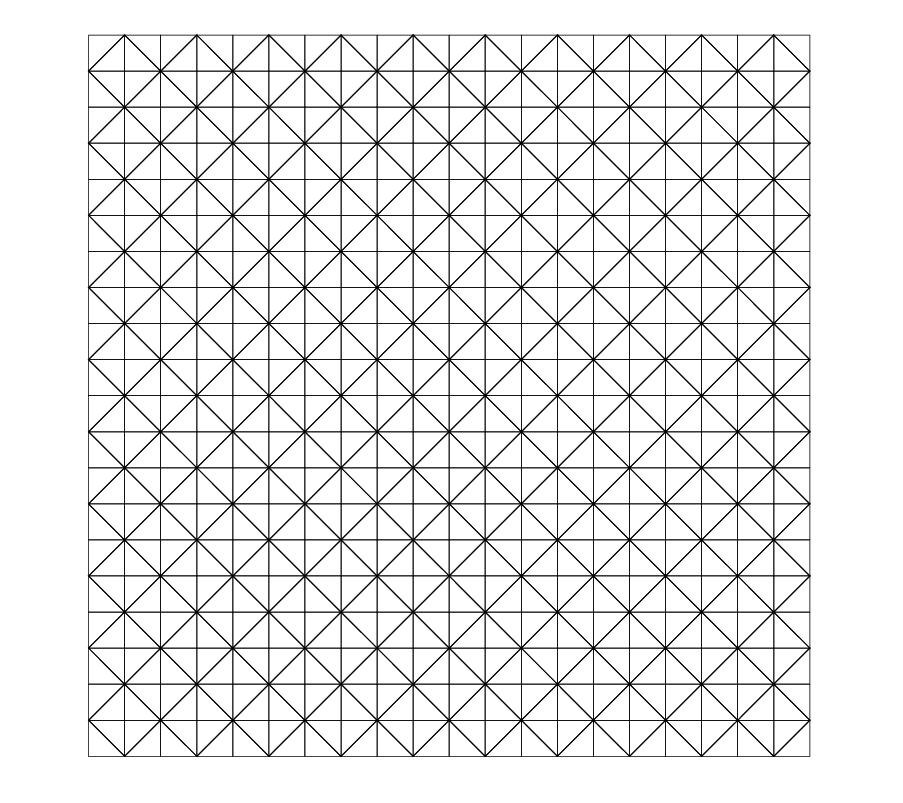
\includegraphics[width=.45\linewidth]{./figs/rect20.png}
    % \label{fig:}
    % \caption{Scottish 类型的规则非结构网格}
  \end{subfigure}%
  % \begin{subfigure}{.3\textwidth}
  \begin{subfigure}
    \centering
    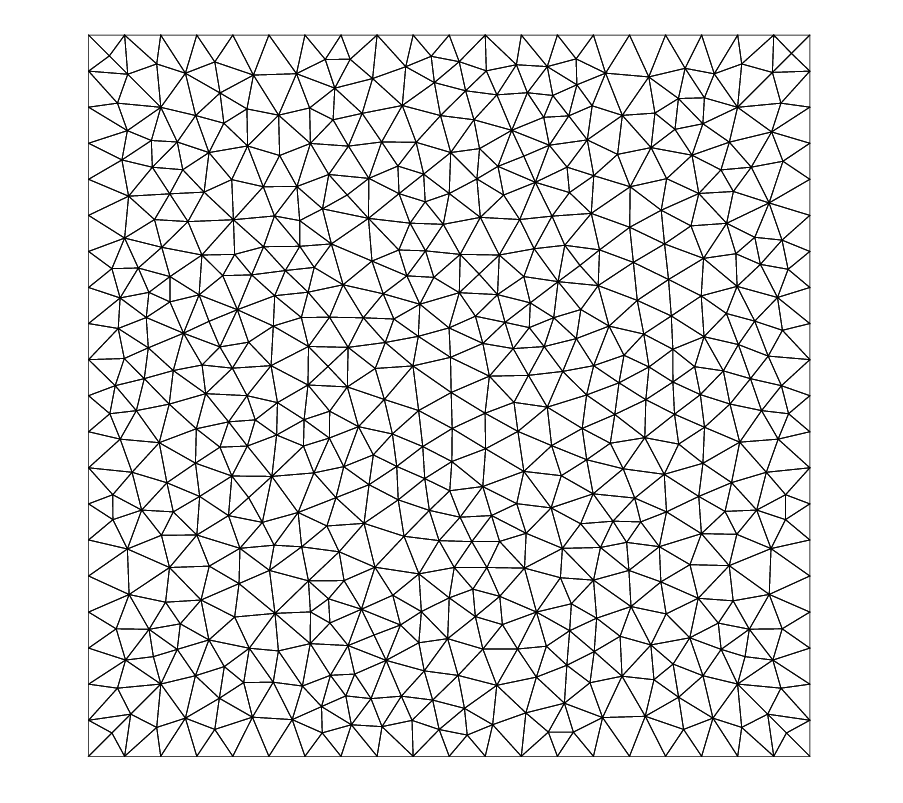
\includegraphics[width=.45\linewidth]{./figs/gmsh20.png}
    % \caption{Delaunay 不规则非结构网格}
  \end{subfigure}
  \caption{两种类型的计算网格}
  \label{fig:computing-grid-compare}
\end{figure}

关于网格是否可以采用周期性边界条件。易知基于矩形网格剖分所得的规则
非结构网格一定满足条件。对于不规则非结构网格,在我们的测试算例
中 GMSH 生成的网格可以通过相应的测试,即可以采用周期性边界条件。

\verb|mesh| 目录下包含如下两个网格相关的工具:
\begin{description}
\item[convert:] 将输入的 \verb|.msh| 文件转化为 EasyMesh 的
  \verb|.e| 和 \verb|.n| 文件。并进行网格的一致性检测。
\item[rect\_trian\_mesh:] 根据需要的网格密度生成基于矩形剖分的三
  角形网格。
\end{description}
用户可以通过 \verb|-h| 命令获得相关工具的详细说明。相应的源代码位
于\verb|./mesh/src| 目录下。在 \verb|./mesh| 下执行 \verb|make|
即可进行编译。

\section{使用方法}
\label{sec:how-to-use}
\begin{enumerate}
\item 修改 \verb|main.cc| 中的相关参数。例如
  \begin{itemize}
  \item cfl 条件数 \verb|cfl|
  \item 结束时间 \verb|t_end|
  \item 网格文件 (不包含后缀名) \verb|mesh_file|
  \item 输出文件 \verb|outfile|
  \item 设定测试算例 \verb|test_suite_type|。测试算例类型参考
    \verb|def.h| 中的 \verb|TEST_SUITE_TYPE|。
  \item 设定初始梯度估计方式 \verb|grad_predicter|。
  \item 设定限制子的计算方法 \verb|grad_limiter|。
  \end{itemize}
\item 执行 \verb|make 2d-unstr-fvm-adv| 生成可执行文件 \verb|2d-unstr-fvm-adv|。
\item 运行程序,输出数据文件,格式为 tec360(tecplot) 的 \verb|.dat| 文件格
  式。
\end{enumerate}

\section{测试算例}
\label{sec:test-case}
考虑线性波问题
\begin{equation}
  \label{eq:linear-wave-problem}
  u_{t} + {\bf{a}} \cdot \nabla u = 0.
\end{equation}
设定速度向量 ${\bf{a}} = (1,2)$ 为常量。 初值为 Double-sine wave
\begin{equation}
  \label{eq:double-sine-wave}
  u_{0} = \sin(2\pi x) \sin(2\pi y), \quad (x,y) \in [0,1] \times[0,1].
\end{equation}
该初值常用于测试方法的收敛阶。网格使用 $80\times80$ 的规则非结构
网格。

\begin{lstlisting}[style=CPP,breaklines=false]
int
main(int argc, char *argv[]){

   FLOAT cfl = 0.5;
   RK_TYPE rk_type = RK_TYPE_2;
   FLOAT t_end = 1.0;
   INT max_time_step = 10000;

   std::string mesh_file("./mesh/rect_trian_80");
   std::string outfile("./dat/test.dat");
   TEST_SUITE_TYPE test_suite_type = TEST_SUITE_TYPE_ADV_DOUBLESINE;

   FLOAT L1_error;

   /* ---- Generate Grid. ---- */

   GRID grid;
   grid.ReadGridFile(mesh_file + ".e", mesh_file + ".n");
   grid.Precondition();
   PERIODIC_BOUNDARY boundary(&grid);
   boundary.ExpendBoundary();

   /* ---- Create solution ---- */

   SOLUTION solution(&grid, &boundary);

   /* ---- Construct the reconstructer ---- */

   GRAD_PREDICT_LS grad_predicter(&solution);
   GRAD_LIMITER_MLP grad_limiter(&solution);
   MUSCL_RECON recon(grad_predicter, grad_limiter, solution);

   /* ---- Set testing case ---- */

   TEST_SUITE test_suite(test_suite_type);

   /* ---- Initialize Solver ---- */

   SOLVER solver(solution,
                 recon,
                 rk_type,
                 cfl,
                 // functors
                 test_suite.ptr_init_function,
                 test_suite.ptr_flux_function,
                 test_suite.ptr_field_function,
                 test_suite.ptr_exact_function
      );

   solver.ShowSolverInfo();

   /* ---- Advance in time ---- */

   solver.AdvanceSolution(t_end, max_time_step);

   /* ---- L1 error ---- */

   std::cout << "Calculating the L1 error ..." << std::endl;
   L1_error = solver.GetL1Error();
   std::cout << std::scientific;
   std::cout << std::setprecision(3);
   std::cout << "L1 error: " << L1_error << std::endl;
   std::cout << std::flush;

   /* ---- Peak ---- */

   std::cout << "Calculation the Peak ..." << std::endl;
   FLOAT max_peak, min_peak;
   std::cout << std::fixed;
   std::cout << std::setprecision(3);
   solver.GetPeak(max_peak, min_peak);
   std::cout << "Max: " << max_peak << std::endl;
   std::cout << "Min: " << min_peak << std::endl;
   std::cout << std::flush;

   /* ---- Output final profile ---- */

   solution.ExportTecplot(outfile);

   return 0;
} /* main */
\end{lstlisting}


\bibliographystyle{abbrv}
\bibliography{./bib/ref}%
\end{document}